As a software system is enhanced, modified, and adapted to new requirements, the code becomes more complex and drifts away from its original design, thereby lowering the quality of the software. {\em Refactoring}~\cite{1999:RID,Griswold:1992,Opdyke1992:ROF,Mens2004:SSR} copes with increasing software complexity by transforming a program from one representation to another while preserving the program's external behavior (functionality and semantics). Mens et al.~present a survey of refactoring research and describe a refactoring process, consisting of the following activities~\cite{Mens2004:SSR}:
\begin{enumerate}
\item Identifying where to apply what refactoring(s).
\item Checking that the refactoring to apply preserves program behaviors.
\item Refactoring the code.
\item Assessing the effect of applied refactoring on software quality (e.g., complexity and readability). 
\item Maintaining the consistency between refactored code and other related software artifacts, like documentation, tests, and issue tracking records.  
\end{enumerate}

Section~\ref{sec:refactoringdefinition} describes the definition of refactoring and example transformations. Section~\ref{sec:refactoringstudies} describes empirical studies on refactoring. Section~\ref{sec:automatedrefactoring} describes tool support for automated refactoring. Section~\ref{sec:refactoringpractice} describes several studies of modern refactoring practices and the limitations of current refactoring support. Section~\ref{sec:refactoringassessment} describes techniques for assessing the impact of refactoring. Section~\ref{sec:codesmell} describes techniques for identifying opportunities for refactoring. 

\subsubsection{Definition of Refactoring Operations.} 
\label{sec:refactoringdefinition} 

Griswold's dissertation \cite{Griswold:1992} discusses one of the first refactoring operations that automate repetitive, error-prone, non-local transformations. Griswold supports a number of restructuring operations: replacing an expression with a variable that has its value, swapping the formal parameters in a procedure's interface and the respective arguments in its calls, etc. It is important to note that many of these refactoring operations are systematic in the sense that they involve repetitive non-local transformations. 

Opdyke's dissertation \cite{Opdyke1992:ROF} distinguishes the notion of low-level refactorings from high-level refactorings. High-level refactorings (i.e., composite refactorings) reflect more complex behavior-preserving transformations while low-level refactorings are primitive operations such as creating, deleting, or changing a program entity or moving a member variable. Opdyke describes three kinds of complex refactorings in detail: (1) creating an abstract superclass, (2) subclassing and simplifying conditionals, and (3) capturing aggregations and components. All three refactorings are systematic in the sense that they contain multiple similar transformations at a code level. For example, {creating an abstract superclass} involves moving multiple variables and functions common to more than one sibling classes to their common superclass.  {Subclassing and simplifying conditionals} consists of creating  several classes, each of which is in charge of evaluating a different conditional. Capturing aggregations and components usually involves moving {multiple} members from a component to an aggregate object. 

While refactoring is defined as behavior-preserving code transformations in the academic literature~\cite{Mens2004:SSR}, the de-facto definition of refactoring in practice seems to be very different from such rigorous definition. Fowler catalogs 72 types of structural changes in object oriented programs but these transformations do not necessarily guarantee behavior preservation~\cite{1999:RID}. In fact, Fowler recommends developers to write test code first, since these refactorings may change a program's behavior. Murphy-Hill et al.~analyzed refactoring logs and found that developers often interleave refactorings with other behavior-modifying transformations~\cite{Murphy-Hill2012:refactor}, indicating that pure refactoring revisions are rare. Johnson's refactoring definition is aligned with these findings\textemdash{\it refactoring improves behavior in some aspects but does not necessarily preserve behavior in all aspects}~\cite{Johnson2011}.

\subsubsection{Empirical Studies of Refactoring.} 
\label{sec:refactoringstudies} 

Hindle et al. found that large commits are more refactorings, while small commits are more bug fixes~\cite{Hindle2008:largecommit}. Purushothaman and Perry found that nearly 10\% of changes involved only a single line of code, which has less than a 4\% chance to result in error, while a change of 500 lines or more has nearly a 50\% chance of causing at least one defect. This result may indicate that large commits, which tend to include refactorings, have a higher chance of inducing bugs. 

Wei{\ss}gerber and Diehl found that refactorings often occur together with other types of changes and that refactorings are followed by an increasing number of bugs~\cite{Weissgerber2006:refactor}. Carriere et al.~found that the productivity measure manifested by the average time taken to resolve tickets decreases after re-architecting the system~\cite{Carriere2010:architecture}. Ratzinger et al.~developed defect prediction models based on software evolution attributes and found that refactoring related features and defects have an inverse correlation~\cite{Ratzinger2008:refactor}\textemdash if the number of refactorings increases in the preceding time period, the number of defects decreases. Kim et al.~investigated the spatial and temporal relationship between API refactorings and bug fixes using a K-revision sliding window and by reasoning about the method-level location of refactorings and bug fixes. They found that the number of bug fixes increases after API refactorings~\cite{Kim2011:refactorbug}.  

Though the intent of refactoring is to improve software maintainability, refactoring could be potentially error-prone as it often requires coordinated edits across different parts of a system. Several researchers found such evidence from open source project histories\textemdash Kim et.al.~found exceptions to systematic change patterns, which often arise from the failure to complete coordinated refactorings~\cite{Kim2007,Kim:2009}. G{\"o}rg and Wei{\ss}gerber detect errors caused by incomplete refactorings by relating API-level refactorings to the corresponding class hierarchy~\cite{Gorg2005a}. Nagappan and Ball found that code churn\textemdash the number of added, deleted, and modified lines of code\textemdash is correlated with defect density~\cite{Nagappan2005}\textemdash since refactoring often introduces a large amount of structural changes to the system, some question the benefit of refactoring. 

\subsubsection{Automated Refactoring.} 
\label{sec:automatedrefactoring} 

The Eclipse IDE provides automatic support for a variety of refactorings, including \emph{rename}, \emph{move}, and \emph{extractMethod}. With such support, developers do not need to worry about how to check for preconditions or postconditions before manually applying a certain refactoring. Instead, they can simply select the refactoring command from a menu (e.g., \emph{extractMethod}), and provide necessary information to accomplish the refactoring (e.g., \emph{the name of a new method}). The Eclipse refactoring engine takes care of the precondition check, program transformation, and post-condition check. 

During refactoring automation, Opdyke suggests to ensure behavior preservation by specifying \emph{refactoring preconditions}~\cite{Opdyke1992:ROF}. For instance, when conducting an \emph{create\_method\_function} refactoring, before inserting a member function $F$ to a class $C$, developers should specify and check for five preconditions, as shown in Figure~\ref{fig:preconditions}. If any precondition is not satisfied, the refactoring should not be applied to the program.

\begin{figure}[!htb]
\centering
\scalebox{0.55}{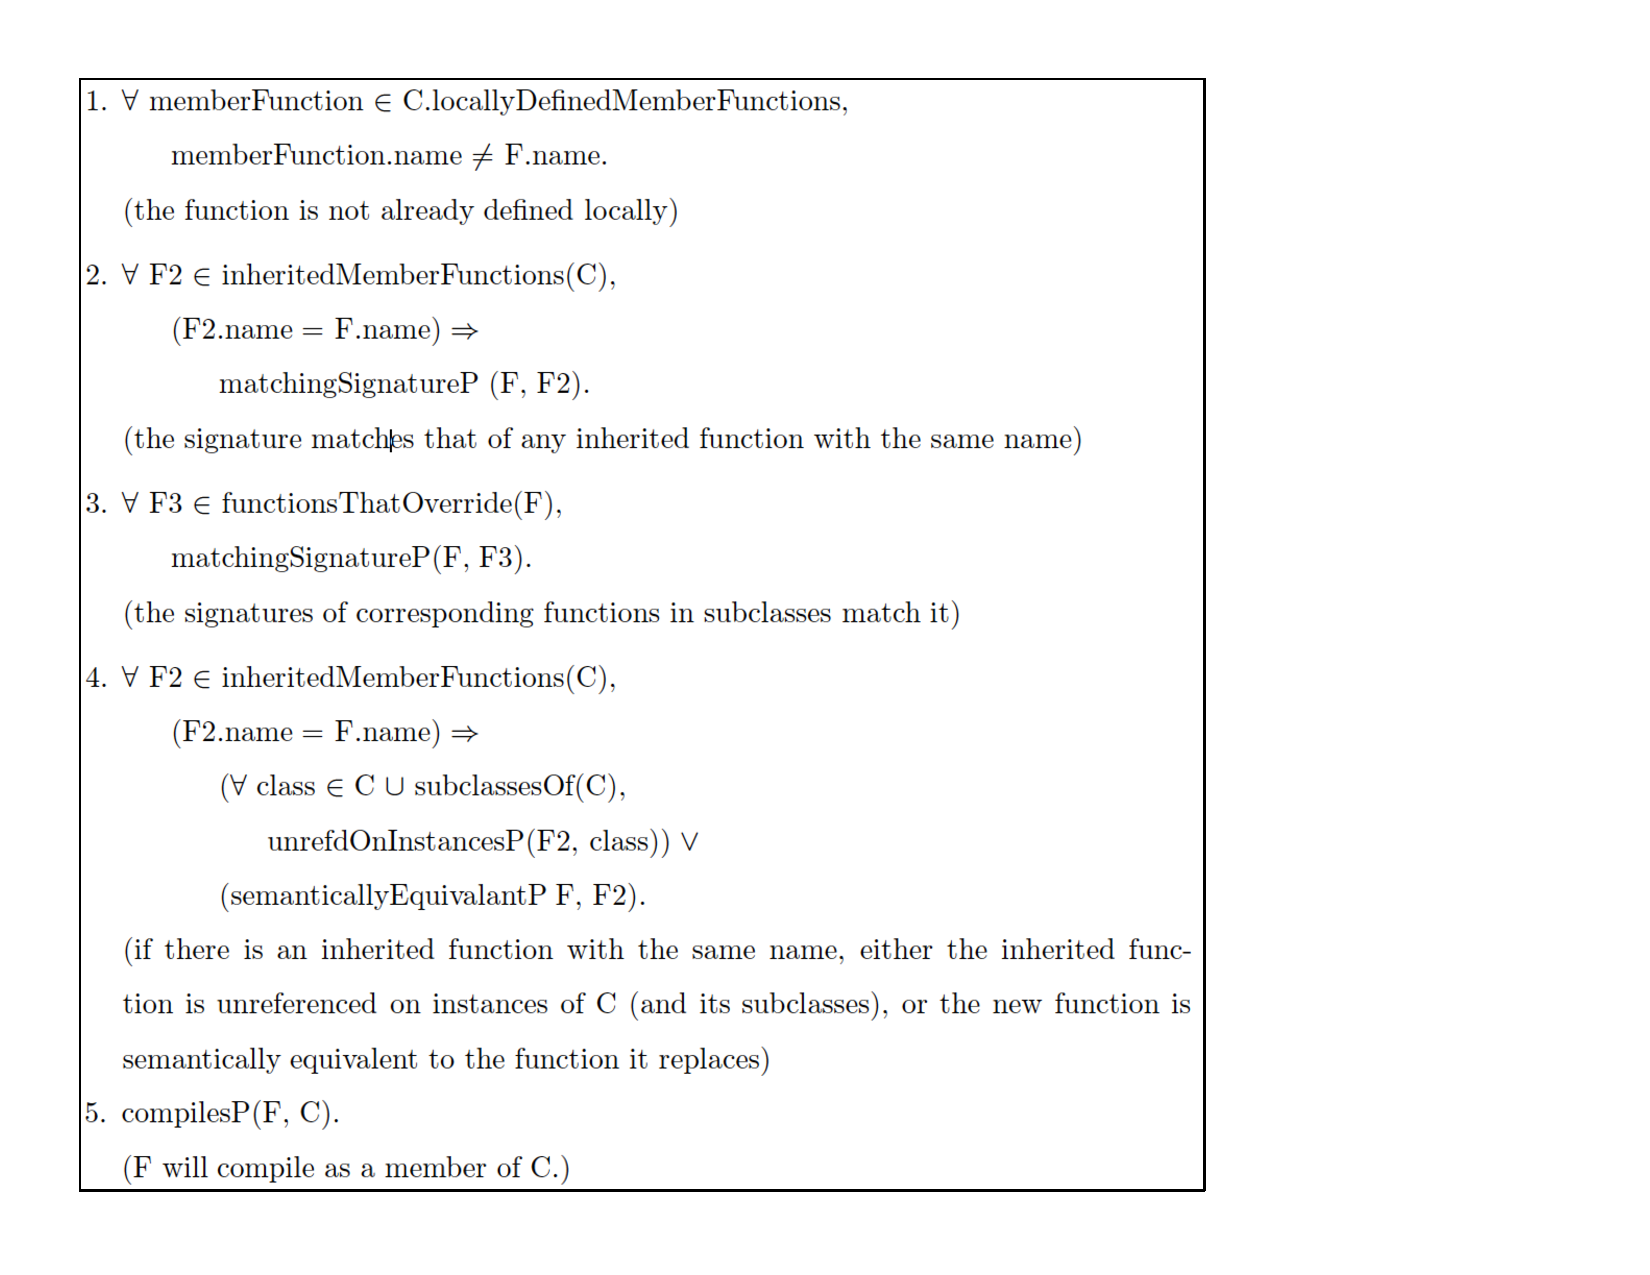
\includegraphics{images/preconditions.pdf}}
\caption{Preconditions for \emph{create\_method\_function} refactoring~\cite{Opdyke1992:ROF}}
\label{fig:preconditions}
\end{figure}

%Additionally, researchers conducted empirical studies to characterize the refactorings applied by developers~\cite{Kim2012:FSR,Murphy-Hill2012:refactor,Vakilian:2012,Silva2016:WWR}, and proposed various approaches to automate refactoring or to complete the refactoring tasks initiated by developers~\cite{Griswold:1992,Balazinska1999,Dig:2009,Ge:2012,Chen:2013,Lee:2013,Tsantalis2013:icsm,Meng2015:ARO,Kim:2016}. For instance, Silva et al.~observed that refactoring activity is mainly driven by changes in the requirements and much less by code smells~\cite{Silva2016:WWR}. Kim et al.~developed R3, an alternative refactoring engine that works 10 times faster than Eclipse Refactoring~\cite{Kim:2016}. 

%Based on code clones detected by various techniques~\cite{Kamiya2002,Jiang2007a,Krinke2001:PDG}, many tools identify or rank refactoring opportunities~\cite{Balazinska1999a, Higo2008:metricrefactoring, goto2013extract, higo2013identifying, Tsantalis2011:rankRefactoring}. For instance, Balazinska et al.~\cite{Balazinska1999a} define a clone classification scheme based on various types of differences between clones and automate the classification to help developers assess refactoring opportunities for each clone group. Higo et al.~and Goto et al.\/ rank clones as refactoring candidates based on coupling or cohesion metrics~\cite{Higo2008:metricrefactoring,goto2013extract}. Others integrate evolution information in software history to rank clones that have been repetitively or simultaneously changed in the past~\cite{higo2013identifying, Tsantalis2011:rankRefactoring}. While these tools detect refactoring opportunities for clones, they do not automatically refactor code.
Clone removal refactorings factorizes the common parts of similar code by parameterizing their differences using a {\em strategy} design pattern or a {\em form template method} refactoring~\cite{Balazinska1999, tairas2012increasing, juillerat2007toward, hotta2012identifying, Tsantalis2013:icsm}. These tools insert customized calls in each original location to use newly created methods. Juillerat et al.~automate {\em introduce exit label} and {\em introduce return object} refactorings~\cite{juillerat2007toward}. However, for variable and expression variations, they define extra methods to mask the differences~\cite{Balazinska1999}. Hotta et al.~use program dependence analysis to handle gapped clones---trivial differences inside code clones that are safe to factor out such that they can apply the {\em form template method} refactoring to the code~\cite{hotta2012identifying}. Krishnan et al.~use PDGs of two programs to identify a maximum common subgraph so that the differences between the two programs are minimized and fewer parameters are introduced~\cite{Tsantalis2013:icsm}. RASE is an advanced clone removal refactoring technique that (1) extracts common code; (2) creates new types and methods as needed; (3) parameterizes differences in types, methods, variables, and expressions; and (4) inserts return objects and exit labels based on control and data flow by combining multiple kinds of clone removal transformations~\cite{Meng2015:ARO}. Such clone removal refactoring could lead to an increase in the total size of code because it creates numerous simple methods. 

%\todo{Na: Tsantalis's new work on clone removal from ICSE 2017 using lambda??} 

Komondoor et al.\/ extract methods based on the user-selected or tool-selected statements in one method~\cite{Komondoor2000, Komondoor2003}. The {\em extract method} refactoring in the Eclipse IDE requires contiguous statements, whereas their approach handles non-contiguous statements. Program dependence analysis identifies the relation between selected and unselected statements and determines whether the non-contiguous code can be moved together to form extractable contiguous code. Komondoor et al.\/ apply {\em introduce exit label} refactoring to handle exiting jumps in selected statements~\cite{Komondoor2003}. Tsantalis et al.\/ extend the techniques by requiring developers to specify a variable of interest at a specific point only~\cite{tsantalis2011identification}. They use a block-based slicing technique to suggest a program slice to isolate the computation of the given variable. These automated procedure extraction approaches are focused on extracting code from a single method only. Therefore, they do not handle extracting common code from multiple methods and resolving the differences between them. 

\subsubsection{Real-World Refactoring Practices.} 
\label{sec:refactoringpractice} 

Several studies investigated refactoring practices in industry and also examine the current challenges and risks associated with refactoring. Kim et al.~conducted a survey with professional developers at Microsoft~\cite{Kim2012:FSR, Kim2014:EmpiricalStudy}. They sent a survey invitation to 1290 engineers whose commit messages include a keyword ``refactoring'' in the version histories of five MS products. 328 of them responded to the survey. More than half of the participants said they carry out refactorings in the context of bug fixes or feature additions, and these changes are generally not semantics-preserving. When they asked about their own definition of refactoring, 46\% of participants did not mention preservation of semantics, behavior, or functionality at all. 53\% reported that refactorings that they perform do not match the types and capability of transformations supported by existing refactoring engines. 

\begin{figure}[!htb]
\centering
    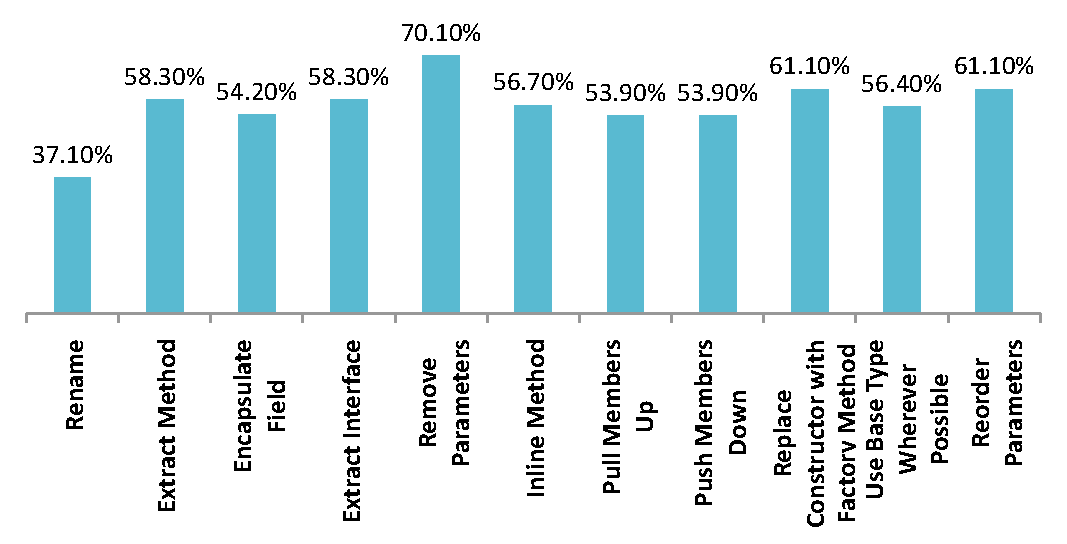
\includegraphics[width=0.55\textwidth]{images/manualRefactoring.pdf}
    \caption{The percentage of survey participants who know individual refactoring types but do those refactorings manually.\cite{Kim2014:EmpiricalStudy}}  
\label{fig:manualRefactoring} 
\end{figure} 

In the same study, when developers are asked {\it ``what percentage of your refactoring is done manually as opposed to using automated refactoring tools?''}, developers answered they do 86\% of refactoring manually on average. Figure~\ref{fig:manualRefactoring} shows the percentages of developers who usually apply individual refactoring types manually despite the awareness of automated refactoring tool support. Vakilian et al.~\cite{Vakilian:2012} and Murphy et al.~\cite{Murphy2006:JSD} also find that programmers do not use automated refactoring despite their awareness of the availability of automated refactorings. Murphy-Hill manually inspected source code produced by 12 developers and found that developers only used refactoring tools for 10\% of refactorings for which tools were available~\cite{Murphy-Hill2012:refactor}. For the question, {\it ``based on your experience, what are the risks involved in refactorings?''}, developers reported regression bugs, code churn, merge conflicts, time taken from other tasks, the difficulty of doing code reviews after refactoring, and the risk of over-engineering. 77\% think that refactoring comes with a risk of introducing subtle bugs and functionality regression~\cite{Kim2012:FSR}.

In a separate study of refactoring tool use, Murphy-Hill et al.~gave developers specific examples of when they did not use refactoring tools, but could have~\cite{Murphy-Hill2012:refactor} and asked why. One reason was that developers started a refactoring manually, but only partway through realized that the change was a refactoring that the IDE offered\textemdash by then, it was too late.  Another complaint was that refactoring tools disrupted their workflow, forcing them to use a tool when they wanted to focus on code.  

\subsubsection{Quantitative Assessment of Refactoring Impact.} 
\label{sec:refactoringassessment} 
While several prior research efforts have conceptually advanced the benefit of refactoring through metaphors, few empirical studies assessed refactoring impact quantitatively. Sullivan et al.~first linked software modularity with option theories~\cite{Sullivan1998:option}. A module provides an option to substitute it with a better one without symmetric obligations, and investing in refactoring activities can be seen as purchasing \emph{options} for future adaptability, which will produce benefits when changes happen and the module can be replaced easily. Baldwin and Clark argued that the modularization of a system can generate tremendous value in an industry, given that this strategy creates valuable options for module improvement~\cite{Baldwin1999:designrule}. Ward Cunningham drew the comparison between debt and a lack of refactoring: a quick and dirty implementation leaves {\em technical debt} that incur \emph{penalties} in terms of increased maintenance costs~\cite{Cunningham1992:td}. While these projects advanced conceptual understanding of refactoring impact, they did not quantify the benefits of refactoring.  

Kim et al.~studied how refactoring impacts inter-module dependencies and defects using the quantitative analysis of Windows 7 version history~\cite{Kim2014:EmpiricalStudy}. Their study finds the top 5\% of preferentially refactored modules experience higher reduction in the number of inter-module dependencies and several complexity measures but increase size more than the bottom 95\%. Based on the hypothesis that measuring the impact of refactoring requires multi-dimensional assessment, they investigate the impact of refactoring on various metrics: churn, complexity, organization and people, cohesiveness of ownership, test coverage and defects.     

MacCormack et al.~defined modularity metrics and used these metrics to study evolution of Mozilla and Linux. They found that the redesign of Mozilla resulted in an architecture that was significantly more modular than that of its predecessor. Their study monitored design structure changes in terms of modularity metrics without identifying the modules where refactoring changes are made~\cite{MacCormack2006:study}. Kataoka et al.~proposed a refactoring evaluation method that compares software before and after refactoring in terms of coupling metrics~\cite{Kataoka2002:metric}. Kolb et al.~performed a case study on the design and implementation of existing software and found that refactoring improves software with respect to maintainability and reusability~\cite{Kolb2006:refactoring}. Moser et al.~ conducted a case study in an industrial, agile environment and found that refactoring enhances quality and reusability related metrics~\cite{Moser2006:refactoring}. Tahvildari et al.~suggested using a catalogue of object-oriented metrics to estimate refactoring impact, including complexity metrics, coupling metrics, and cohesion metrics~\cite{Tahvildari2003:MAE}. 

\subsubsection{Code Smells Detection.} 
\label{sec:codesmell} 

Fowler describes the concept of {\em bad smell} as a heuristic for identifying redesign and refactoring opportunities~\cite{1999:RID}. Example bad smells include code clone and feature envy. Several techniques automatically identify bad smells that indicate needs of refactorings~\cite{Tsantalis2009:extractmethod,Tsantalis2009:movemethod,Tsantalis2008:jdeodorant}. 

Garcia et al.~propose several architecture-level bad smells~\cite{Garcia2009:badsmell}. Moha et al.~present the Decor tool and domain specific language (DSL) to automate the construction of design defect detection algorithms~\cite{Moha2009:designdefect}. 
Tsantalis and Chatzigeorgiou's technique identifies {\em extract method} refactoring opportunities using static slicing~\cite{Tsantalis2009:extractmethod}. Detection of some specific bad smells such as code duplication has also been extensively researched. Higo et al.~propose the Aries tool to identify possible refactoring candidates based on the number of assigned variables, the number of referred variables, and dispersion in the class hierarchy~\cite{Higo2004}. A refactoring can be suggested if the metrics for the clones satisfy certain predefined values. 
Koni-N'Sapu provides refactoring suggestions based on the location of clones with respect to a class hierarchy~\cite{koni_nsapu:ms01}. Balazinska et al.~suggest clone refactoring opportunities based on the differences between the cloned methods and the context of attributes, methods, and classes containing clones~\cite{Balazinska2000:ACA}. Kataoka et al.~use Daikon to infer program invariants at runtime, and suggest candidate refactorings using inferred invariants~\cite{Kataoka2001:ASP}. If Daikon observes that one parameter of a method is always constant, it then suggests a \emph{removeParameter} refactoring. {\it Breakaway} automatically identifies detailed structural correspondences between two abstract syntax trees to help programmers generalize two pieces of similar code~\cite{Cottrell:2007}. 

Gueheneuc et al.~detect inter-class design defects~\cite{Gueheneuc2001:designdefect} and Marinescu identifies design flaws using software metrics~\cite{Marinescu2004:designflaw}. Izurieta and Bieman detect accumulation of non design-pattern related code~\cite{Izurieta2007:grime}. Guo et al.~define domain-specific code smells~\cite{Guo2010:smell} and investigate the consequence of technical debt~\cite{Guo2011:td}. Tsantalis et al.~rank clones that have been repetitively or simultaneously changed in the past to suggest refactorings~\cite{Tsantalis2011:rankRefactoring}. Wang et al.~extract features from code to reflect program context, code smell, and evolution history, and then use a machine learning technique to rank clones for refactorings~\cite{Wang2014:recommendClones}.

Clio detects modularity violations based on the assumptions that multiple types of bad smells are instances of modularity violations that can be uniformly detected by reasoning about modularity hierarchy in conjunction with change locations~\cite{Wong2011:cleo}. They define {\em modularity violations} as recurring discrepancies between which modules should change together and which modules actually change together according to version histories. For example, when code clones change frequently together, Clio will detect this problem because the co-change pattern deviate from the designed modular structure. Second, by taking version histories as input, Clio detects violations that happened most recently and frequently, instead of bad smells detected in a single version without regard to the program's evolution context. Ratzinger et al.~also detect bad smells by examining change couplings but their approach leaves it to developers to identify design violations from visualization of change coupling~\cite{ratzinger:msr05}. 

%Related to the problem of code smells detection, various approaches have been proposed to automatically suggest refactoring opportunities based on program context or version history~\cite{Balazinska2000:ACA,Kataoka2001:ASP,Higo2008:metricrefactoring,Tsantalis2011:rankRefactoring,Wang2014:recommendClones,Meng2015:ARO}. Specifically,
%Balazinska et al.~used a clone detection tool to identify duplicated code and to suggest clone removal refactorings~\cite{Balazinska2000:ACA}. 

